\documentclass[10pt]{article}
\usepackage[T1]{fontenc}
\usepackage[utf8]{inputenc}
\usepackage[english,russian]{babel}
\usepackage{xcolor}
\usepackage{listings}
\usepackage{hyperref}
\usepackage{float}
\usepackage{fancyhdr}
\usepackage{graphicx}
\usepackage{textcmds}

\definecolor{dkgreen}{rgb}{0,0.6,0}
\definecolor{lghtgray}{rgb}{0.97,0.97,0.97}
\definecolor{gray}{rgb}{0.5,0.5,0.5}
\definecolor{kwblue}{rgb}{0.2,0.6,1.0}

\lstdefinestyle{lua}{
  defaultdialect=[5.0]Lua,
  deletekeywords={type},
  frame=single,
  language=Lua,
  aboveskip=3mm,
  belowskip=3mm,
  showstringspaces=false,
  columns=flexible,
  backgroundcolor=\color{lghtgray},
  basicstyle={\small\ttfamily},
  numbers=left,
  numberstyle=\footnotesize\color{black},
  keywordstyle=\color{kwblue}\bfseries,
  commentstyle=\color{dkgreen},
  stringstyle=\color{brown},
  breaklines=true,
  breakatwhitespace=true,
  tabsize=4,
  extendedchars=false,
  inputencoding=utf8
}

\lstset{style=lua}

\usepackage{geometry}
 \geometry{
 a4paper,
 total={170mm,257mm},
 left=20mm,
 top=20mm,
 }

\usepackage{hyperref}
\hypersetup{
    colorlinks=true,
    linkcolor=teal,   
    urlcolor=blue,
    }


% In case you want watermark on each page!
%\usepackage{draftwatermark}
%\SetWatermarkText{Черновик}
%\SetWatermarkScale{2}
%\SetWatermarkColor{red}


\author{mak}
\title{\selectlanguage{Russian}Генератор случайных сценариев Disciples 2\\Документация для версии 0.8.0}

\begin{document}
\pagestyle{fancy}
 % clear all header fields
\fancyhead{}
 % clear all footer fields
\fancyfoot{}
% page number in the center for even and odd pages
\fancyfoot[CE,CO]{\thepage}
\fancyhead[RO,RE]{\textcolor{gray}{Версия генератора 0.8.0}}

\maketitle
\newpage
\tableofcontents
\newpage
\listoffigures

\selectlanguage{Russian}
% Differences against previous version
\section{Отличия от версии 0.5.0}
\begin{itemize}
\item в параметры шаблона добавлены поля
\begin{itemize}
\item \texttt{startingNativeMana}
\item \texttt{forbiddenUnits}
\item \texttt{forbiddenItems}
\item \texttt{forbiddenSpells}
\end{itemize}
\item добавлен новый тип данных \texttt{Border}
\item в параметры зоны добавлены поля
\begin{itemize}
\item \texttt{border}
\item \texttt{gapChance}
\end{itemize}
\end{itemize}
% Introduction
\section{Введение}
Генератор сценариев предназначен для создания пользовательских сценариев (карт) со случайным наполнением по шаблонам. Шаблоны представляют собой обычные текстовые файлы на языке \href{https://www.lua.org/}{Lua}.

Задача шаблона - описать содержимое генерируемой карты и задать дефолтные настройки для игрока. Ключевым фактором генерации является создание зон соединенных правильным образом, а также заданного числа объектов, отрядов и наград внутри них максимально близко к указанной ценности. Шаблоны определяют что игрок может ожидать от сценария, какой контент будет присутствовать, при этом никаких гарантий о расположении контента нет. Например: если в зоне указаны 2 лавки торговца и 1 руины значит что они встретятся во время игры, но не обязательно в удобном для игрока месте.

% GUI app usage
\section{Программа генератора}
\subsection{Обзор и установка}
Генератор находится в стадии прототипа и не встроен в игру, поэтому на данный момент представляет собой отдельную программу с графическим интерфейсом. Внешний вид программы генератора после запуска представлен ниже:

\begin{figure}[H]
\center
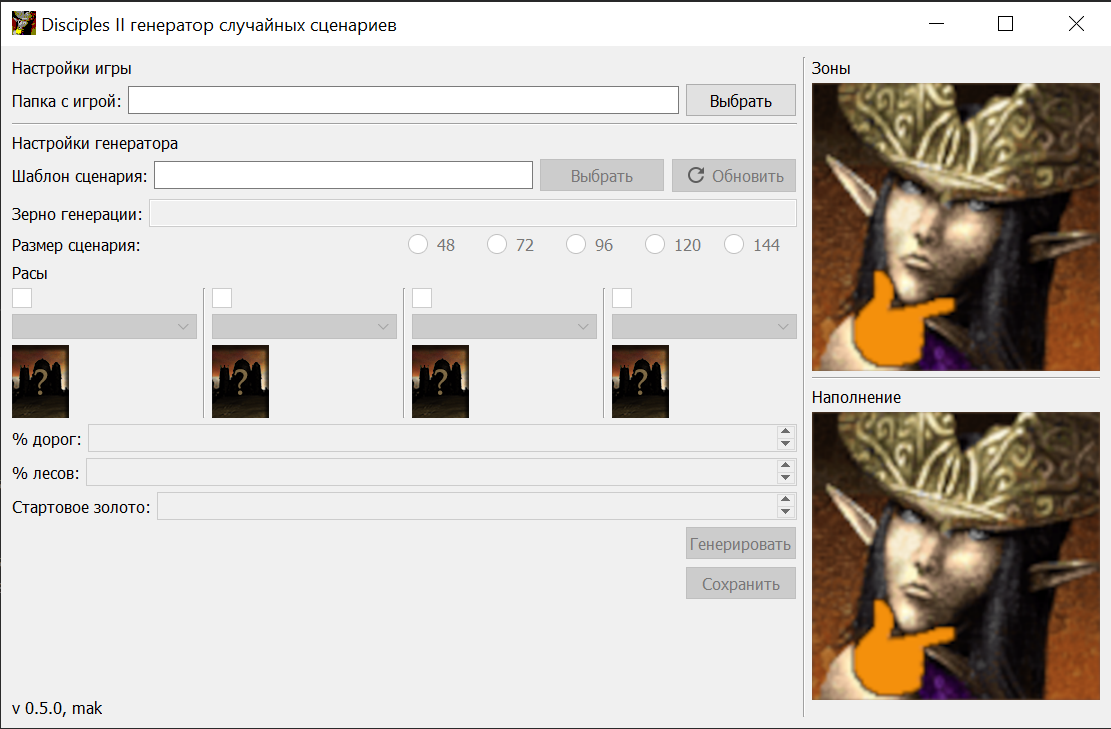
\includegraphics[width=.8\linewidth]{docImages/interface.png}
\caption{Интерфейс программы генератора}
\end{figure}

Генератор не привязан к конкретному моду и, при наличии корректного файла настроек, может работать как с оригинальной Disciples II: Rise of the Elves (v 3.01), так и с любыми модами.

Прототип генератора \textbf{не нуждается} в тулсете для моддинга \href{https://github.com/VladimirMakeev/D2ModdingToolset}{\texttt{mss32.dll}} и работает независимо от его наличия.
Для того чтобы генератор мог корректно создавать сценарии ему необходим файл с настройками \texttt{generatorSettings.lua}, который должен быть помещен в папку \texttt{Scripts} внутри папки с игрой.\\
В данном файле задаются \qq{подсказки} для генератора - информация об игре, которую невозможно определить алгоритмически:
\begin{itemize}
\item списки юнитов и предметов, запрещенных к использованию генератором
\item списки изображений магазинов, башен магов, лагерей наемников, тренеров и руин. Их наземные и водные варианты
\item списки лендмарок (Landmarks) наиболее подходящих визуально для расположения на территориях игровых рас, нейтральной территории, а также выглядящих как горы
\end{itemize}

Данный подход позволяет генератору не зависеть от особенностей модификации игры, но давая возможность настроить баланс и визуальную части генерации ценой одного дополнительного файла на языке \href{https://www.lua.org/}{Lua}.

Вместе с программой генератором и этой документацией идут заранее подготовленные файлы настроек \texttt{generatorSettings.lua} для PvP-модов \href{https://norvezskayasemga.pro/}{sMNS (v1.0.1.2+)} и \href{https://drive.google.com/drive/folders/1RKBPSrk6SC4viXzhdPFkUHgwEqOl3WeT}{Мотлина (v 1.5.3+)}. Перед использованием генератора файлы настроек, как было сказано ранее, необходимо закинуть в папку \texttt{Scripts} внутри папки с игрой.

\newpage
\subsection{Генерация сценария по шаблону}
Интерфейс программы сделан с целью минимизации ошибок со стороны пользователя во время использования. Недоступные в данный момент кнопки и элементы становятся неактивными и активируются когда их использование возможно.\\
Типичный вариант использования программы:
\begin{itemize}
\item Выбор папки с игрой. В верхней части интерфейс в строке \texttt{"Папка с игрой"} необходимо нажать кнопку \texttt{"Выбрать"} и выбрать \textbf{папку} игры
\item Если файл настроек генератора был заранее добавлен в папку \texttt{Scripts} внутри папки игры, должна стать доступна опция выбора шаблона сценария напротив строки \texttt{"Шаблон сценария"}
\item После выбора шаблона станет доступна кнопка \texttt{"Обновить"}, она будет полезна при разработке и тестировании шаблона. См. \hyperref[templateDevelopment]{\selectlanguage{Russian}Разработка шаблона} 
\item После выбора шаблона будут доступны опции влияющие на создаваемый сценарий. Они будут подробно рассмотрены далее
\item Также, внизу станет доступна кнопка \texttt{"Генерировать"}, которая запустит сам процесс генерации с учетом содержимого шаблона и выбранных пользователем опций генерации
\item Во время генерации интерфейс станет неактивен во избежание смены настроек посреди процесса генерации
\item По окончании генерации интерфейс снова станет активен, а также станет доступна кнопка \texttt{"Сохранить"} для записи результатов генерации в файл сценария \texttt{(.sg)} на жестком диске.
\item Для удобства пользователей и авторов шаблонов справа в окне программы находятся две области предпросмотра: просмотр расположения зон и "миникарта" с данными об их наполнении. Области автоматически обновляются после каждой успешной генерации сценария
\end{itemize}

\newpage
\subsection{Опции генерации}
\label{templateOptions}
Опции генерации сценария представляют собой те настройки шаблона, которые автор разрешил пользователям менять. Таким образом значения по умолчанию и некоторые параметры целиком зависят от шаблона. Программа генератора лишь выводит их в интерфейс для удобства выбора пользователем.
Опции генерации сценария:\\
\begin{itemize}
\item Зерно генерации - целое число определяющее зерно для генератора случайных чисел, используемого при создании сценария. \textbf{Важно:} генератор обладает свойством воспроизводимости. При использовании одинаковой версии генератора, мода и его версии, шаблона, зерна генерации, размера сценария, списка рас, \% дорог и лесов результаты генерации будут полностью идентичны и воспроизводимы
\item Размер сценария - размер игровой карты в тайлах. Доступные для выбора пользователя размеры зависят от шаблона и определяются его автором
\item Расы - можно выбрать определенные расы, либо случайную, предоставив генератору сделать выбор. Генератор не создает сценарии, нарушающие правила и механики игры, поэтому выбрать две одинаковые расы не получится. Одинаковые расы также никогда не будут созданы в случае выбора случайных рас. Создание и использование шаблонов явно задающих две и более одинаковых рас в стартовых зонах приведет к ошибкам генерации. Возможность выбора меньшего числа рас, чем указано в шаблоне, на данный момент не реализована
\item \% дорог - генератор располагает интерактивные объекты внутри зон так чтобы каждый из них был доступен для посещения отрядами игрока. К каждому из объектов генератор проведет "проходы" или "тропы" которые не будут заняты непроходимыми препятствиями. Процент дорог определяет какой процент тайлов проходов будет также содержать тайлы игровых дорог, дающих бонус к движению наземных отрядов
\item \% лесов - в процессе наполнения сценария генератор помечает будущие тайлы как \qq{свободные}, \qq{занятые} или \qq{возможные}. \qq{Возможные} тайлы возможно будут заняты, а возможно свободны. Процент лесов определяет сколько \qq{возможных} тайлов, оставшихся после наполнения сценария объектами, будут отданы под лес
\item Стартовое золото - количество бонусного золота с которым каждый из игроков начнет сценарий
\end{itemize}

\newpage
\subsection{Разработка шаблона}
\label{templateDevelopment}
При создании и тестировании нового шаблона часто возникает необходимость быстро проверять вносимые в шаблон правки. Специально для этого используется кнопка \texttt{"Обновить"}, которая перезагрузает файл шаблона с диска без необходимости его повторного выбора в диалоговом окне. \hyperref[templateOptions]{\selectlanguage{Russian}Опции генерации} автоматически обновляются и корректируются при перезагрузке, а следующая генерация сценария будет учитывать внесенные правки сокращая время между тестами. Обновлять файл шаблона можно любое число раз.

\subsection{Процесс генерации и шаблон}
В виду особенностей игровых механик (расы, источники маны, субрасы и свободный проход мимо "родных" отрядов нейтралов) возникла необходимость связать выбор игрока перед началом генерации и содержимое шаблона. В следствие этого шаблон сценария содержит одновременно описательную часть и динамическое содержимое.\\
Описательная часть - название, опции генерации видимые игроку в интерфейсе генератора (в дальнейшем и в интерфейсе игры).\\
Динамическое содержимое - зоны, их наполнение объектами с учетом выбранных пользователем рас и размеров карты, а также проходы между зонами. Динамическое содержимое в файле шаблона описывается и возвращается функцией \texttt{getContents}, которая будет вызвана с учетом параметров пользователя после нажатия кнопки \texttt{"Генерировать"}.\\
Генератор загружает и показывает пользователю описательную часть ожидая изменений в опциях. При запуске генерации измененные опции будут использованы для интерпретации динамического содержимого шаблона и непосредственной генерации сценария.
% Template format description
\section{Формат файла шаблона}
Шаблоном считается любой корректный файл на языке \href{https://www.lua.org/}{Lua} в котором присутствует таблица \texttt{template} с параметрами для игрока, а также полем-функцией \texttt{getContents}, которая принимает список рас и размер сценария. Функция \texttt{getContents} должна вернуть таблицу с содержимым шаблона, его контентом. Поле \texttt{zones} в возвращаемой таблице содержит список зон и их объектов, а поле \texttt{connections} определяет связи (проходы) между зонами и опциональную охрану.

\subsection{Параметры видимые игроку}
Для удобства игрока шаблон определяет несколько параметров которые могут быть изменены пользователем по своему желанию перед генерацией сценария. Такие параметры как \texttt{name} и \texttt{description} не изменяемы и служат лишь для описания шаблона, а также подсказок игроку о возможном содержимом.

\subsubsection{Параметры шаблона}
\begin{itemize}
\item \texttt{name} - название шаблона
\item \texttt{description} - описание шаблона
\item \texttt{minSize} - минимальный размер сценария какой может быть создан этим шаблоном. 48 по умолчанию, максимум 144
\item \texttt{maxSize} - максимальный размер сценария какой может быть создан этим шаблоном. 48 по умолчанию, максимум 144
\item \texttt{maxPlayers} - количество игроков (рас) в сценарии. 1 по умолчанию, максимум 4
\item \texttt{startingGold} - количество бонусного золота для каждого игрока. 0 по умолчанию, максимум 9999
\item \texttt{startingNativeMana} - количество бонусной родной маны для каждого игрока. 0 по умолчанию, максимум 9999
\item \texttt{roads} - процент тайлов проходов которые станут дорогами дающими бонус передвижения. Диапазон \texttt{[0 : 100]}, 100 по умолчанию
\item \texttt{forest} - процент неиспользованных тайлов которые станут лесом. Диапазон \texttt{[0 : 100]}, 0 по умолчанию

\item \texttt{forbiddenUnits} - список идентификаторов юнитов запрещенных для генерации на шаблоне.
Идентификаторы юнитов можно найти в \texttt{GUnits.dbf} или программе
\href{https://drive.google.com/file/d/1hI7OYhoQbeizglwZwY8UuWSSr6Q1i6WO/view}{Disciples2Info}.
Запрещенных юнитов можно добавить в \hyperref[mercenary]{\selectlanguage{Russian}лагеря наемников} явно указав их в списке обязательных.

\item \texttt{forbiddenItems} - список идентификаторов предметов запрещенных для генерации на шаблоне.
Идентификаторы вещей можно найти в \texttt{GItems.dbf}.
Запрещенные предметы можно добавить в \hyperref[loot]{\selectlanguage{Russian}награды} явно указав их в списке обязательных предметов.

\item \texttt{forbiddenSpells} - список идентификаторов заклинаний запрещенных для генерации в \hyperref[mage]{\selectlanguage{Russian}Башнях магов} на шаблоне.
Идентификаторы заклинаний можно найти в \texttt{GSpells.dbf}.
Запрещенные заклинания можно добавить в \hyperref[mage]{\selectlanguage{Russian}Башни магов} явно указав их в списке обязательных заклинаний.

\item \texttt{customParameters} - список с описанием дополнительных параметров шаблона. См. \hyperref[customParameters]{\selectlanguage{Russian}Дополнительные параметры шаблона}.
\end{itemize}

\subsection{Описание содержимого}
\label{contentsTable}
Для удобства игроков и авторов шаблонов содержимое шаблона может зависеть от настроек игрока. Основными параметрами являются список рас и размер сценария.
Так же передается список выбранных значений для дополнительных параметров.
Список рас позволит контролировать субрасы отрядов, награды и тип рудников, а размер сценария даст возможность масштабировать количество объектов и отрядов.
Таким образом одним шаблоном можно описать правила генерации чтобы сценарии были играбельны как на размере 48, так и 144.\\
Описание содержимого шаблона создает функция \texttt{getContents}, которая принимает три аргумента:
\begin{itemize}
\item \texttt{races} - список рас, заданных игроком или выбранных случайно. См. \hyperref[raceTypes]{\selectlanguage{Russian}Расы}
\item \texttt{scenarioSize} - размер сценария, выбранный игроком перед началом генерации
\item \texttt{customParameters} - список значений, выбранных для дополнительных параметров. См. \hyperref[customParameters]{\selectlanguage{Russian}Дополнительные параметры шаблона}.
\end{itemize}
Функция должна вернуть таблицу содержимого - настройки зон, их наполнение и связи между ними. На основании содержимого генератор создает сценарий.\\
Обязательные поля таблицы:
\begin{itemize}
\item \texttt{zones} - список зон. См. \hyperref[zone]{\selectlanguage{Russian}Зона}
\item \texttt{connections} - список соединений зон. См. \hyperref[connection]{\selectlanguage{Russian}Проход}
\end{itemize}
Необязательные поля:
\begin{itemize}
\item \texttt{diplomacy} - список дипломатических отношений между расами. См. \hyperref[diplomacy]{\selectlanguage{Russian}Дипломатия}
\end{itemize}

\subsection{Пример}
Ниже показан пример простейшего шаблона который создаст пустой сценарий с одной зоной, занимающей всю карту, а также одним игроком. Раса игрока зависит от выбора пользователя.
Формат описания содержимого, зон, соединений и объектов подробно рассматривается в следующей секции.
\begin{figure}[H]
\lstinputlisting{docExamples/example.lua}
\caption{\selectlanguage{Russian}Простейший шаблон}
\end{figure}
% Key concepts and data types
\section{Ключевые понятия}
Зоны, их содержимое, а также соединения между зонами описываются с помощью Lua таблиц.
Простейшая таблица в языке Lua выглядит следующим образом:\\
\begin{lstlisting}
{ }
\end{lstlisting}
Таблицы могут быть пустыми, либо содержать именованые поля, не именованые поля и другие таблицы:
Пустая таблица:\\
\begin{lstlisting}
{ }
\end{lstlisting}
Таблица с именоваными полями:\\
\begin{lstlisting}
{ min = 0, max = 100 }
\end{lstlisting}
Таблица с полями без имен, используются индексы (начиная с 1):\\
\begin{lstlisting}
{ [1] = 1, [2] = 100 }
\end{lstlisting}
Таблица с двумя вложенными таблицами:\\
\begin{lstlisting}
{ { min = 0, max = 100 }, { min = 10, max = 50 } }
\end{lstlisting}
Для удобства чтения таблицы могут быть сохранены в переменные, тем самым получая имя:
\begin{lstlisting}
local emptyTable = {}
\end{lstlisting}


Вложенность таблиц и их полей важна, а порядок задания полей не играет роли.\\
Таким образом приведенный выше пример шаблона содержит таблицу \texttt{template} с полями
\texttt{name}, \texttt{description}, \texttt{roads}, \texttt{forest} и другими.
Также, поле \texttt{getContents} в таблице \texttt{template} указывает на функцию которая возвращает безымянную таблицу 
содержащую 2 именованых поля \texttt{zones} и \texttt{connections}, которые в свою очередь также являются таблицами.
Для удобства чтения этот блок кода можно было записать иначе:
\begin{figure}[h]
\lstinputlisting{docExamples/getContents.lua}
\caption{\selectlanguage{Russian}Вариант написания функции \texttt{getContents}}
\end{figure}

\newpage
% Describe common data types and enumerations used by generator
\subsection{Типы данных}
В случае с описанием содержимого шаблона генератор понимает и ожидает некоторые заранее определенные таблицы и данные. Поля внутри таких таблиц зависят от того что описывает таблица, другими словами её типа. Ниже будут подробно рассмотрены все существующие типы таблиц, их назначение и поля.

\subsubsection{Расы}
\label{raceTypes}
Расы известные генератору:
\begin{itemize}
\item \texttt{Race.Human} - Защитники Империи
\item \texttt{Race.Undead} - Орды нежити
\item \texttt{Race.Heretic} - Легионы проклатых
\item \texttt{Race.Dwarf} - Горные кланы
\item \texttt{Race.Elf} - Альянс эльфов
\item \texttt{Race.Neutral} - Нейтралы
\end{itemize}
\textbf{\selectlanguage{Russian}Важно:} нейтралы не могут появиться в списке рас функции \texttt{getContents}.

\subsubsection{Субрасы}
\label{subraceTypes}
Субрасы известные генератору:
\begin{itemize}
\item \texttt{Subrace.Human} - Защитники Империи
\item \texttt{Subrace.Undead} - Орды нежити
\item \texttt{Subrace.Heretic} - Легионы проклятых
\item \texttt{Subrace.Dwarf} - Горные кланы
\item \texttt{Subrace.Elf} - Альянс эльфов
\item \texttt{Subrace.Neutral} - Нейтралы
\item \texttt{Subrace.NeutralHuman} - Нейтральные люди
\item \texttt{Subrace.NeutralElf} - Нейтральные эльфы
\item \texttt{Subrace.NeutralGreenSkin} - Зеленокожие
\item \texttt{Subrace.NeutralDragon} - Драконы
\item \texttt{Subrace.NeutralMarsh} - Жители болот
\item \texttt{Subrace.NeutralWater} - Водные обитатели
\item \texttt{Subrace.NeutralBarbarian} - Варвары
\item \texttt{Subrace.NeutralWolf} - Животные
\item \texttt{Subrace.Custom} - Своя субраса
\end{itemize}

\subsubsection{Типы предметов}
\label{itemTypes}
Типы предметов известные генератору:
\begin{itemize}
\item \texttt{Item.Armor} - Артефакты (не влияющие на урон)
\item \texttt{Item.Jewel} - Реликвии
\item \texttt{Item.Weapon} - Артефакты (влияющие на урон)
\item \texttt{Item.Banner} - Знамена
\item \texttt{Item.PotionBoost} - Зелья бафов
\item \texttt{Item.PotionHeal} - Зелья лечения
\item \texttt{Item.PotionRevive} - Зелья воскрешения
\item \texttt{Item.PotionPermanent} - Зелья дающие постоянный эффект
\item \texttt{Item.Scroll} - Свитки
\item \texttt{Item.Wand} - Посохи
\item \texttt{Item.Valuable} - Драгоценности
\item \texttt{Item.Orb} - Сферы
\item \texttt{Item.Talisman} - Талисманы
\item \texttt{Item.TravelItem} - Походное снаряжение
\item \texttt{Item.Special} - Особые
\end{itemize}

\subsubsection{Типы заклинаний}
\label{spellTypes}
Типы заклинаний известные генератору:
\begin{itemize}
\item \texttt{Spell.Attack} - Наносящие урон, например 'Армагеддон'
\item \texttt{Spell.Lower} - Снижающие показатели (дебафы), например 'Гниение'
\item \texttt{Spell.Heal} - Лечащие заклинания, например 'Исцеление'
\item \texttt{Spell.Boost} - Увеличивающие показатели (бафы), например 'Гимн Кланов'
\item \texttt{Spell.Summon} - Призыв, например 'Вызов Белиарха'
\item \texttt{Spell.Fog} - Наложение тумана войны, например 'Сумерки'
\item \texttt{Spell.Unfog} - Открытие тумана войны, например 'Свет дня'
\item \texttt{Spell.RestoreMove} - Восстановление очков движения, например 'Подвижность'
\item \texttt{Spell.Invisibility} - Невидимость, например 'Сокрытие'
\item \texttt{Spell.RemoveRod} - Удаление жезлов, например 'Водосточный колодец'
\item \texttt{Spell.ChangeTerrain} - Смена типа поверхности, например 'Создание Рощи'
\item \texttt{Spell.GiveWards} - Наложение даров (вардов), например 'Влиятельность' (Мотлин), 'Поспешность' (MNS)
\end{itemize}
\newpage
% Describe zone types and their behavior
\subsection{Типы зон}
\label{zoneTypes}
Типы зон поддерживаемые генератором:
\begin{itemize}
\item \texttt{Zone.PlayerStart} - стартовая локация игрока. В центре зоны появится столица указанной расы. Первый рудник золота и источник родной маны будут под контролем расы.
\item \texttt{Zone.Treasure} - сокровищница или обычная зона. В зоне будет создано множесто случайных проходов между объектами, выходами, а также ведущие в тупик.
\item \texttt{Zone.Junction} - проходная, соединительная зона. Будет создан один проход соединяющий выходы.
\end{itemize}
\newpage
% Describe all supported tables and their fields
\subsection{Типы таблиц}

% Zone description
\subsubsection{Зона}
\label{zone}
Определяет зону на карте сценария.

Обязательные поля:
\begin{itemize}
\item \texttt{id} - идентификатор зоны. Число, уникально определяющее зону
\item \texttt{type} - тип зоны. См. \hyperref[zoneTypes]{\selectlanguage{Russian}Типы зон}
\item \texttt{size} - относительный размер зоны
\end{itemize}

В случае если в качестве типа зоны выбрана стартовая локация \texttt{type = Zone.PlayerStart}, нужно указать уникальную расу для игрока в этой зоне:
\begin{itemize}
\item \texttt{race} - раса игрока. Одна из поданного в \texttt{getContents} списка рас или заранее заданная. См. \hyperref[raceTypes]{\selectlanguage{Russian}Расы}
\end{itemize}

Необязательные поля:
\begin{itemize}
\item \texttt{mines} - источники ресурсов в зоне. См. \hyperref[crystals]{\selectlanguage{Russian}Источники ресурсов}
\item \texttt{towns} - список нейтральных городов. См. \hyperref[city]{\selectlanguage{Russian}Город}
\item \texttt{ruins} - список руин. См. \hyperref[ruin]{\selectlanguage{Russian}Руины}
\item \texttt{merchants} - список торговцев. См. \hyperref[merchant]{\selectlanguage{Russian}Торговец}
\item \texttt{mages} - список башен магов. См. \hyperref[mage]{\selectlanguage{Russian}Башня мага}
\item \texttt{mercenaries} - список лагерей наемников. См. \hyperref[mercenary]{\selectlanguage{Russian}Лагерь наемников}
\item \texttt{trainers} - список тренировочных лагерей. См. \hyperref[trainer]{\selectlanguage{Russian}Тренер}
\item \texttt{stacks} - список групп нейтральных отрядов в зоне. См. \hyperref[neutralStacks]{\selectlanguage{Russian}Нейтральные отряды}
\item \texttt{bags} - неохраняемые сундуки в зоне. См. \hyperref[bags]{\selectlanguage{Russian}Неохраняемые сундуки}
\end{itemize}

Для стартовых локаций игроков также возможно задание гарнизона, предметов в столице и заклинаний известных игроку со старта:
\begin{itemize}
\item \texttt{capital} - столица игрока. См. \hyperref[capital]{\selectlanguage{Russian}Столица}
\end{itemize}

Примеры:\\
Стартовая зона с относительным размером 20. Здесь будет столица первого игрока из списка рас.
В зоне будут созданы 1 золотой рудник и 1 источник маны рун.

\begin{figure}[H]
\lstinputlisting{docExamples/zoneExample1.lua}
\end{figure}

Стартовая зона с относительным размером 20. Здесь будет столица первого игрока из списка рас.
Независимо от выбранной расы, в гарнизоне столице будут созданы юниты империи общей ценностью 150 - 175.
В инвентаре столицы будут созданы зелья лечения и воскрешения ценностью 750 - 800.
Игроку-владельцу со старта будут известны заклинания 'Ледяной щит' и 'Молния'.

\begin{figure}[H]
\lstinputlisting{docExamples/zoneExample2.lua}
\end{figure}

Обычная зона (сокровищница) с относительным размером 35.
В зоне будут случайно расположены 12 нейтральных отрядов общей ценностью 1200 - 1300,
а также 5 нейтральных отрядов общей ценностью 2000.

\begin{figure}[H]
\lstinputlisting{docExamples/zoneExample3.lua}
\end{figure}
\newpage
% Connection description
\subsubsection{Проход}
\label{connection}
Определяет соединение двух зон, проход между ними.
Между двумя зонами может быть более одного прохода.

Обязательные поля:
\begin{itemize}
\item \texttt{from} - идентификатор первой зоны. См. \hyperref[zone]{\selectlanguage{Russian}Зона}
\item \texttt{to} - идентификатор второй зоны. См. \hyperref[zone]{\selectlanguage{Russian}Зона}
\end{itemize}

Необязательные поля:
\begin{itemize}
\item \texttt{guard} - отряд охраняющий проход между зонами. См. \hyperref[group]{\selectlanguage{Russian}Группа / Отряд}
\end{itemize}

Примеры:\\
Проход между зонами 0 и 1, без охраны
\begin{figure}[h]
\lstinputlisting{docExamples/connectionExample1.lua}
\end{figure}

Проход между зонами 1 и 0, аналогичен предыдущему примеру
\begin{figure}[h]
\lstinputlisting{docExamples/connectionExample2.lua}
\end{figure}

Проход между зонами 0 и 3.
Охраняется отрядом ценностью 1750 - 2250.
В инвентаре отряда будут созданы артефакты, знамена или перманентные зелья общей ценностью 2500 - 3000
\begin{figure}[h]
\lstinputlisting{docExamples/connectionExample3.lua}
\end{figure}
\newpage
% Diplomacy relations description
\subsubsection{Дипломатия}
\label{diplomacy}
Определяет дипломатические отношения между двумя расами.

Обязательные поля:
\begin{itemize}
\item \texttt{raceA} - первая раса. См. \hyperref[raceTypes]{\selectlanguage{Russian}Раса}
\item \texttt{raceB} - вторая раса. См. \hyperref[raceTypes]{\selectlanguage{Russian}Раса}
\item \texttt{relation} - уровень отношений в диапазоне \texttt{[0 : 100]}. 0 - вражда, 100 - мир
\end{itemize}
Необязательные поля:
\begin{itemize}
\item \texttt{alliance} - \texttt{true} если расы находятся в союзе. Не может быть \texttt{true} когда \texttt{alwaysAtWar} также \texttt{true}. По умолчанию \texttt{false}
\item \texttt{alwaysAtWar} - \texttt{true} если расы находятся в состоянии вечной вражды. Не может быть \texttt{true} когда \texttt{alliance} также \texttt{true}. По умолчанию \texttt{false}
\item \texttt{permanentAlliance} - \texttt{true} если альянс считается постоянным для ИИ. Не может быть \texttt{true} когда \texttt{alliance} \texttt{false}. По умолчанию \texttt{false}
\end{itemize}

Примеры:\\
Две расы находятся в состоянии вражды:

\begin{figure}[H]
\lstinputlisting{docExamples/diplomacyExample1.lua}
\end{figure}

Две расы находятся в состоянии вражды, заключение союза невозможно:

\begin{figure}[H]
\lstinputlisting{docExamples/diplomacyExample2.lua}
\end{figure}

Две расы находятся в союзе. ИИ не может расторгнуть союз:

\begin{figure}[H]
\lstinputlisting{docExamples/diplomacyExample3.lua}
\end{figure}
\newpage
% Value description
\subsubsection{Ценность}
\label{value}
Задает ценность группы (отряда), юнита, предмета или заклинания в диапазоне \texttt{[min : max]}.

Расчет ценности генератором сценариев:
\begin{itemize}
\item ценность групп, отрядов и юнитов определяется их опытом за убийство, значение \texttt{XP\_KILLED} из GUnits.dbf
\item ценность предметов определяется как сумма всех ресурсов в стоимости их покупки у торговца, значение \texttt{VALUE} из GItems.dbf
\item ценность заклинаний определяется как сумма всех ресурсов в стоимости их покупки в башне мага, значение \texttt{BUY\_C} из GSpells.dbf
\end{itemize}

Сумма всех ресурсов:\\
К примеру предмет \texttt{А} стоит 100 золота и 50 маны жизни. Сумма всех ресурсов его стоимости даст ценность равную 150.
Предмет \texttt{Б} стоит 150 золота. Его ценность, также как у \texttt{А}, будет 150.\\
Для генератора золото и все типы маны равноценны.

Обязательные поля:
\begin{itemize}
\item \texttt{min} - минимальное значение ценности. Целое число
\item \texttt{max} - максимальное значение ценности. Целое число
\end{itemize}

Примеры:\\
Ценность от 100 до 200 включительно:\\
\begin{lstlisting}
{ min = 100, max = 200 }
\end{lstlisting}
Ценность 175:\\
\begin{lstlisting}
{ min = 175, max = 175 }
\end{lstlisting}
\newpage
% Loot item description
\subsubsection{Предмет награды}
\label{item}
Описывает обязательный предмет в награде.

Обязательные поля:
\begin{itemize}
\item \texttt{id} - идентификатор предмета из GItems.dbf
\item \texttt{min} - минимальное число предметов
\item \texttt{max} - максимальное число предметов
\end{itemize}

Пример:\\
От 1 до 5 эликсиров восстановления\\
\begin{lstlisting}
{ id = 'g000ig0006', min = 1, max = 5 }
\end{lstlisting}
\newpage
% Loot description
\subsubsection{Награда}
\label{loot}
Описывает награду (лут). Награда может состоять из случайных и обязательных предметов.

Обязательных полей нет, пустая таблица создаст пустую награду.

Необязательные поля:
\begin{itemize}
\item \texttt{value} - ценность случайных предметов в награде. См. \hyperref[value]{\selectlanguage{Russian}Ценность}
\item \texttt{itemValue} - диапазон ценности каждого случайного предмета в награде. См. \hyperref[value]{\selectlanguage{Russian}Ценность}
\item \texttt{itemTypes} - список типов случайных предметов которые могут быть созданы. В случае пустого списка может быть создан предмет любого типа, кроме специального \texttt{Item.Special}
\item \texttt{items} - список предметов которые обязательно должны быть созданы. Не зависит от ценности награды. См. \hyperref[item]{\selectlanguage{Russian}Предмет награды}
\end{itemize}

Примеры:\\
Случайная награда из зелий-бафов и воскрешения общей стоимостью от 500 до 750,
а также от 3 до 5 эликсиров восстановления

\begin{figure}[H]
\lstinputlisting{docExamples/lootExample1.lua}
\end{figure}

Награда из 5 зелий восстановления

\begin{figure}[H]
\lstinputlisting{docExamples/lootExample2.lua}
\end{figure}

Случайная награда из знамен и сапог общей стоимостью от 2500 до 2750

\begin{figure}[H]
\lstinputlisting{docExamples/lootExample3.lua}
\end{figure}

Случайная награда общей стоимостью от 1600 до 1800 
из зелий лечения или воскрешения каждое стоимостью от 200 до 450. 
Подняв минимальную ценность каждой случайной вещи до 200 
мы исключаем дешевые зелья лечения (50 hp) из награды.

\begin{figure}[H]
\lstinputlisting{docExamples/lootExample4.lua}
\end{figure}
\newpage
% Group / Stack description
\subsubsection{Группа / Отряд}
\label{group}
Описывает группу юнитов в руинах или гарнизоне города, либо отряд с лидером.

Обязательные поля:
\begin{itemize}
\item \texttt{value} - общая ценность юнитов. См. \hyperref[value]{\selectlanguage{Russian}Ценность}
\end{itemize}

Необязательные поля:
\begin{itemize}
\item \texttt{subraceTypes} - список сабрас определяющий какие типы юнитов могут быть созданы. См. \hyperref[subraceTypes]{\selectlanguage{Russian}Субрасы}. В случае пустого списка могут быть созданы юниты любых субрас
\item \texttt{loot} - награда. См. \hyperref[loot]{\selectlanguage{Russian}Награда}. В случае отряда награда создаст предметы инвентаря. Для группы в гарнизоне города награда создаст предметы в городе. \textbf{\selectlanguage{Russian}Важно:} награда группы внутри руин \textbf{\selectlanguage{Russian}не учитывается!}. Награда руин задается отдельно. См. \hyperref[ruin]{\selectlanguage{Russian}Руины}
\end{itemize}

Пример:\\
Группа / Отряд из гномов или нейтральных людей.
В качестве награды будут созданы зелья лечения и бафов на 200 - 300 ценности.

\begin{figure}[H]
\lstinputlisting{docExamples/groupExample.lua}
\end{figure}
\newpage
% City description
\subsubsection{Город}
\label{city}
Описывает нейтральный город, его гарнизон и посещающий отряд, а также предметы внутри города.

Обязательные поля:
\begin{itemize}
\item \texttt{tier} - уровень города в диапазоне \texttt{[1: 5]}
\end{itemize}

Необязательные поля:
\begin{itemize}
\item \texttt{garrison} - защитники в гарнизоне города. См. \hyperref[group]{\selectlanguage{Russian}Группа / Отряд}. \textbf{\selectlanguage{Russian}Важно:} Предметы указанные для защитников будут созданы в инвентаре города.
\item \texttt{stack} - отряд посещающий город. См. \hyperref[group]{\selectlanguage{Russian}Группа / Отряд}
\end{itemize}

Пример:\\
Город 1 уровня с гарнизоном из гномов или нейтральных людей.
В гарнизоне будут созданы зелья лечения и бафов на 200 - 300 ценности.
Посещающий отряд в воротах города состоит из варваров и волков.

\begin{figure}[H]
\lstinputlisting{docExamples/cityExample.lua}
\end{figure}
\newpage
% Capital description
\subsubsection{Столица}
\label{capital}
Описывает столицу в стартовой зоне под контролем игрока. Из-за особенностей игры, описание столицы совпадает с описанием городов лишь частично.

Обязательных полей нет, пустая таблица создаст столицу со стражем, но без стартовых предметов. Стартовые зоны игроков всегда будут содержать столицы в своих центрах.

Необязательные поля:
\begin{itemize}
\item \texttt{garrison} - защитники в гарнизоне столицы. См. \hyperref[group]{\selectlanguage{Russian}Группа / Отряд}. \textbf{\selectlanguage{Russian}Важно:} независимо от ценности и субрас гарнизона в нем всегда будет создан страж столицы соответствующий расе игрока. \textbf{\selectlanguage{Russian}Важно:} Предметы указанные для защитников будут созданы в инвентаре столицы
\item \texttt{spells} - список идентификаторов заклинаний из \texttt{GSpells.dbf} которые будут известны игроку со старта
\item \texttt{aiPriority} - приоритет столицы для ИИ в диапазоне \texttt{[0 : 6]}
\item \texttt{name} - название столицы. По умолчанию будет использовано название из \texttt{Cityname.dbf}
\item \texttt{guardian} - определяет будет ли сгенерирован страж столицы. По умолчанию true
\item \texttt{gapMask} - блокирует появление объектов и гор с определенных сторон. См. \hyperref[gapMask]{\selectlanguage{Russian}Маска отступа}
\end{itemize}

Пример:\\
Столица с гарнизоном из войск империи.
В инвентаре будут созданы зелья лечения и воскрешения на 750 - 800 ценности.
Игроку-владельцу столицы со старта будут известны 2 заклинания

\begin{figure}[H]
\lstinputlisting{docExamples/capitalExample.lua}
\end{figure}
\newpage
% Ruins description
\subsubsection{Руины}
\label{ruin}
Описывает руины, их защитников и награду.

Обязательные поля:
\begin{itemize}
\item \texttt{guard} - юниты внутри руин. См. \hyperref[group]{\selectlanguage{Russian}Группа / Отряд}. \textbf{\selectlanguage{Russian}Важно:} предметы указанные для этой группы игнорируются!
\end{itemize}

Необязательные поля:
\begin{itemize}
\item \texttt{gold} - награда за руины в золоте. См. \hyperref[value]{\selectlanguage{Russian}Ценность}
\item \texttt{loot} - предмет-награда за руины. См. \hyperref[loot]{\selectlanguage{Russian}Награда}. \textbf{\selectlanguage{Russian}Важно:} только один предмет из награды будет создан. Обязательные предметы имеют приоритет над случайными. В случае обязательных предметов будет выбран первый из списка.
\item \texttt{aiPriority} - приоритет руин для ИИ в диапазоне \texttt{[0 : 6]}
\end{itemize}

Пример:\\
Руины с наградой из эликсира восстановления и 200 - 250 золота.
Охраняются группой защитников империи или нейтральных людей

\begin{figure}[H]
\lstinputlisting{docExamples/ruinExample.lua}
\end{figure}
\newpage
% Merchant description
\subsubsection{Торговец}
\label{merchant}
Описывает лавку торговца, его товары и потенциальную охрану.

Обязательные поля:
\begin{itemize}
\item \texttt{goods} - ассортимент предметов торговца. См. \hyperref[loot]{\selectlanguage{Russian}Награда}. Торговцы в игре не продают драгоценности (\texttt{Item.Valuable}), поэтому генератор \textbf{\selectlanguage{Russian}никогда} не создаст предметы этого типа среди случайных. Если такие предметы по какой-то причине все же необходимы в ассортименте торговца, следует указать их в списке обязательных предметов
\end{itemize}

Необязательные поля:
\begin{itemize}
\item \texttt{guard} - отряд охраняющий вход в лавку торговца. См. \hyperref[group]{\selectlanguage{Russian}Группа / Отряд}
\end{itemize}

Пример:\\
Торговец продающий оружие, броню, посохи и свитки на сумму от 1000 до 1500.
В ассортименте также от 1 до 5 эликсиров восстановления.
Охраняется отрядом защитников империи или нейтральных людей

\begin{figure}[H]
\lstinputlisting{docExamples/merchantExample.lua}
\end{figure}
\newpage
% Mage description
\subsubsection{Башня мага}
\label{mage}
Описывает башню мага, его заклинания и потенциальную охрану. Заклинания делятся на случайные и обязательные.

Обязательных полей нет, пустая таблица описывает башню мага без заклинаний и охраны.

Необязательные поля:
\begin{itemize}
\item \texttt{value} - общая ценность случайных заклинаний. Ценностью заклинания считается стоимость его покупки (сумма всех ресурсов), поле \texttt{BUY\_C} из GSpells.dbf.  См. \hyperref[value]{\selectlanguage{Russian}Ценность}
\item \texttt{spellLevel} - диапазон уровней каждого случайного заклинания. Допустимые значения: \texttt{[1 : 5]}. Если не задано, в башне могут продаваться заклинания любых уровней
\item \texttt{spellTypes} - список типов случайных заклинаний которые могут появиться. См. \hyperref[spellTypes]{\selectlanguage{Russian}Типы заклинаний}. В случае пустого списка могут быть выбраны заклинания любых типов
\item \texttt{spells} - список идентификаторов заклинаний из GSpells.dbf которые обязательно появятся в башне мага.
\item \texttt{guard} - отряд охраняющий вход в башню мага. См. \hyperref[group]{\selectlanguage{Russian}Группа / Отряд}
\item \texttt{aiPriority} - приоритет башни мага для ИИ в диапазоне \texttt{[0 : 6]}
\end{itemize}

Пример:\\
Башня мага с заклинаниями лечения и ускорений общей ценностью от 200 до 1000.
В ассортименте обязательно появятся 'Быстрота' и 'Молния'

\begin{figure}[H]
\lstinputlisting{docExamples/mageExample1.lua}
\end{figure}

Башня мага с заклинаниями только 2 уровня общей ценностью от 2700 до 3000.
Если каждое заклинание 2 уровня стоит порядка 300 золота (ценность 300),
получим примерно 9-10 заклинаний в ассортименте

\begin{figure}[H]
\lstinputlisting{docExamples/mageExample2.lua}
\end{figure}
\newpage
% Mercenary unit description
\subsubsection{Наемник}
\label{mercenaryUnit}
Описывает обязательного наемника в лагере.

Обязательные поля:
\begin{itemize}
\item \texttt{id} - идентификатор юнита из GUnits.dbf
\item \texttt{level} - уровень юнита. \textbf{\selectlanguage{Russian}Важно:} уровень юнита не может быть ниже базового!
\end{itemize}

Необязательные поля:
\begin{itemize}
\item \texttt{unique} - определяет будет ли юнит доступен для найма единожды
\end{itemize}

Пример:\\
'Рейнджер' (т2 лучник империи), доступный для найма бесконечное число раз

\begin{lstlisting}
{ id = 'g000uu0007', level = 2, unique = false }
\end{lstlisting}

'Скелет-воин' (т3 воин нежити) 20 уровня, доступный для найма единожды

\begin{lstlisting}
{ id = 'g000uu0088', level = 20, unique = true }
\end{lstlisting}
\newpage
% Mercenary camp description
\subsubsection{Лагерь наемников}
\label{mercenary}
Описывает лагерь наемников, юнитов в нем, а также потенциальную охрану. Юниты делятся на случайные и обязательные.

Обязательные поля:
\begin{itemize}
\item \texttt{value} - общая ценность случайных юнитов. См. \hyperref[value]{\selectlanguage{Russian}Ценность}
\end{itemize}

Необязательные поля:
\begin{itemize}
\item \texttt{subraceTypes} - список сабрас определяющий какие типы юнитов могут быть созданы. См. \hyperref[subraceTypes]{\selectlanguage{Russian}Субрасы}. В случае пустого списка могут быть созданы юниты любых субрас
\item \texttt{units} - список наемников которые обязательно должны быть в лагере. Не зависит от ценности случайных юнитов. См. \hyperref[mercenaryUnit]{\selectlanguage{Russian}Наемник}
\item \texttt{guard} - отряд охраняющий вход в лагерь. См. \hyperref[group]{\selectlanguage{Russian}Группа / Отряд}
\end{itemize}

Пример:\\
Лагерь наемников с юнитами империи и нейтральными людьми общей ценностью от 200 до 250.
В лагере обязательно будут доступны 'Рейнджер' и 'Скелет-воин' 20 уровня, доступный для найма лишь единожды

\begin{figure}[H]
\lstinputlisting{docExamples/mercenaryExample.lua}
\end{figure}
\newpage
% Trainer description
\subsubsection{Тренер}
\label{trainer}
Описывает тренировочный лагерь и его опциональную охрану.

Обязательных полей нет. Пустая таблица описывает тренировочный лагерь без охраны.

Необязательные поля:
\begin{itemize}
\item \texttt{guard} - отряд охраняющий вход в лагерь. См. \hyperref[group]{\selectlanguage{Russian}Группа / Отряд}
\item \texttt{aiPriority} - приоритет тренера для ИИ в диапазоне \texttt{[0 : 6]}
\item \texttt{name} - название тренера. По умолчанию будет использовано название из \texttt{Trainame.dbf}
\item \texttt{description} - описание тренера. По умолчанию будет использовано описание из \texttt{Trainame.dbf}
\end{itemize}

Пример:\\
Тренировочный лагерь с отрядом охраны из людей и нейтральных людей общей ценностью 200 - 250.

\begin{figure}[H]
\lstinputlisting{docExamples/trainerExample.lua}
\end{figure}
\newpage
% Tradable resource description
\subsubsection{Ресурс рынка}
\label{marketresource}
Описывает один из ресурсов доступный для обмена на рынке.

Обязательные поля:
\begin{itemize}
\item \texttt{resource} - тип ресурса. См. \hyperref[resourceTypes]{\selectlanguage{Russian}типы ресурсов}
\end{itemize}

Необязательные поля:
\begin{itemize}
\item \texttt{value} - количество ресурса, если его запасы конечны. См. \hyperref[value]{\selectlanguage{Russian}Ценность}.
\item \texttt{infinite} - исчерпаемость ресурса. При значении \texttt{true} ресурс бесконечен, а поле \texttt{value} игнорируется.
\end{itemize}

Пример:\\
Золото, бесконечный запас

\begin{lstlisting}
{ resource = Resource.Gold, infinite = true }
\end{lstlisting}

Мана жизни, количество от 200 до 300

\begin{lstlisting}
{ resource = Resource.LifeMana, value = { min = 200, max = 300 } }
\end{lstlisting}
\newpage
% Resource market description
\subsubsection{Рынок ресурсов}
\label{resourcemarket}
Описывает рынок, его обменный курс, запасы ресурсов и потенциальную охрану.

Обязательных полей нет, пустая таблица описывает рынок с обменным курсом по-умолчанию, без ресурсов и охраны.

Необязательные поля:
\begin{itemize}
\item \texttt{exchangeRates} - строка, содержащая скрипт обменного курса, специфичного для рынка.
\item \texttt{stock} - список \hyperref[marketresource]{\selectlanguage{Russian}ресурсов рынка}.
\item \texttt{guard} - отряд охраняющий вход на рынок. См. \hyperref[group]{\selectlanguage{Russian}Группа / Отряд}
\item \texttt{aiPriority} - приоритет рынка для ИИ в диапазоне \texttt{[0 : 6]}
\item \texttt{name} - название рынка. По умолчанию будет использовано название из \texttt{Marketname.dbf}
\item \texttt{description} - описание рынка. По умолчанию будет использовано описание из \texttt{Marketname.dbf}
\end{itemize}

Пример:\\
Рынок с бесконечным запасом золота, 100 единицами маны жизни, 200 - 300 единиц маны преисподней и 500 - 550 единиц маны смерти

\begin{figure}[H]
\lstinputlisting{docExamples/marketExample1.lua}
\end{figure}

Рынок с бесконечным запасом маны и специальным обменным курсом который позволяет игрокам менять золото на любой вид маны в соотношении 10 к 1

\begin{figure}[H]
\lstinputlisting{docExamples/marketExample2.lua}
\end{figure}
\newpage
% Crystals description
\subsubsection{Источники ресурсов}
\label{crystals}
Описывает количество источников ресурсов каждого типа внутри зоны. В случае стартовых зон, первый источник золота и родной для игрока маны будут автоматически под владением игрока этой зоны.

Обязательных полей нет. Пустая таблица описывает зону без источников ресурсов.

Необязательные поля:
\begin{itemize}
\item \texttt{gold} - количество золотых шахт 
\item \texttt{infernalMana} - количество источников маны преисподней
\item \texttt{lifeMana} - количество источников маны жизни
\item \texttt{deathMana} - количество источников маны смерти
\item \texttt{runicMana} - количество источников маны рун
\item \texttt{groveMana} - количество источников лесного эликсира
\end{itemize}

Пример:\\
Зона с тремя золотыми шахтами и одним источником маны каждого вида

\begin{figure}[H]
\lstinputlisting{docExamples/crystalsExample.lua}
\end{figure}
\newpage
% Neutral stacks description
\subsubsection{Нейтральные отряды}
\label{neutralStacks}
Описывает группу из нескольких нейтральных отрядов создаваемых по общему для них описанию.
Нейтральные отряды будут расположены случайным образом внутри зоны и могут блокировать проходы, а также доступ к некоторым объектам.

Обязательных полей нет. Пустая таблица описывает пустую группу нейтральных отрядов.

Необязательные поля:
\begin{itemize}
\item Все поля, описывающие отряд. Ценность и награды будут равномерно распределены по всем отрядам в группе. См. \hyperref[group]{\selectlanguage{Russian}Группа / Отряд}
\item \texttt{count} - количество случайных отрядов в группе
\item \texttt{owner} - раса, контролирующая отряды. По умолчанию отряды принадлежат нейтральной расе. См. \hyperref[raceTypes]{\selectlanguage{Russian}Расы}
\end{itemize}

Примеры:\\
12 случайных отрядов общей ценностью 1200.
Награда из зелий лечения и буста общей ценностью 200 - 300.
На 12 отрядов обязательно будут созданы  1 - 5 эликсиров восстановления.

\begin{figure}[H]
\lstinputlisting{docExamples/neutralStacksExample1.lua}
\end{figure}

5 случайных отрядов из воинов империи и нейтральных людей общей ценностью 1500 - 1600.

\begin{figure}[H]
\lstinputlisting{docExamples/neutralStacksExample2.lua}
\end{figure}
\newpage
% Bags description
\subsubsection{Неохраняемые сундуки}
\label{bags}
Описывает неохраняемые сундуки внутри зоны.

Обязательных полей нет. Пустая таблица описывает зону без сундуков.

Необязательные поля:
\begin{itemize}
\item \texttt{loot} - общая награда всех сундуков. Будет равномерно распределена по всем сундукам. См. \hyperref[loot]{\selectlanguage{Russian}Награда}
\item \texttt{count} - количество сундуков в зоне
\item \texttt{aiPriority} - приоритет сундуков для ИИ в диапазоне \texttt{[0 : 6]}
\end{itemize}

Пример:\\
10 сундуков с зельями на буст и воскрешение общей суммой 5000 - 7500.
На 10 сундуков обязательно будут созданы 15 эликсиров восстановления.

\begin{figure}[H]
\lstinputlisting{docExamples/bagsExample.lua}
\end{figure}
\newpage

% Example of template creation and testing
\section{Пример создания и проверки шаблона}
В качестве примера работы с Lua, таблицами и описаниями объектов из этой документации в следующих разделах мы по шагам создадим простой, по играбельный шаблон сценария. Мы начнем с пустой, но рабочей заготовки и будем постепенно дополнять ее, проверяя резульаты генерации на каждом шагу.

\subsection{Заготовка шаблона}
Воспользуемся заготовкой шаблона приведенной ниже. Код заготовки поставляется вместе с программой генератором и этой документацией.

\begin{figure}[H]
\lstinputlisting{docExamples/templateExample1.lua}
\caption{Заготовка для создания шаблона \texttt{example.lua}}
\end{figure}

Разберем текст заготовки подробно:\\
Наш шаблон будет создавать сценарии размером от 48 до 72, на выбор игрока:
\begin{figure}[H]
\lstinputlisting[firstnumber=4, firstline=4, lastline=5]{docExamples/templateExample1.lua}
\end{figure}

Наш шаблон будет создавать сценарии для двух игроков:

\begin{figure}[H]
\lstinputlisting[firstnumber=6, firstline=6, lastline=6]{docExamples/templateExample1.lua}
\end{figure}

По-умолчанию процент лесов 65:

\begin{figure}[H]
\lstinputlisting[firstnumber=7, firstline=7, lastline=7]{docExamples/templateExample1.lua}
\end{figure}

Также, на 40\% клеток проходов будут созданы тайлы дорог, дающие бонус наземным отрядам:

\begin{figure}[H]
\lstinputlisting[firstnumber=8, firstline=8, lastline=8]{docExamples/templateExample1.lua}
\end{figure}

Бонус по стартовому золоту для обоих игроков по-умолчанию задан в 850:

\begin{figure}[H]
\lstinputlisting[firstnumber=9, firstline=9, lastline=9]{docExamples/templateExample1.lua}
\end{figure}

Функция \texttt{getContents} возвращает таблицу содержающую список из двух зон:

\begin{figure}[H]
\lstinputlisting[firstnumber=13, firstline=13, lastline=26]{docExamples/templateExample1.lua}
\end{figure}

Первая зона в списке имеет \texttt{id} 0. Используя этот номер мы затем сможем задать проход между зонами:

\begin{figure}[H]
\lstinputlisting[firstnumber=15, firstline=15, lastline=15]{docExamples/templateExample1.lua}
\end{figure}

Первая зона является стартовой зоной игрока, там будет расположена столица:

\begin{figure}[H]
\lstinputlisting[firstnumber=16, firstline=16, lastline=16]{docExamples/templateExample1.lua}
\end{figure}

Расы игроков будут выбраны самими игроками перед началом генерации по шаблону, мы лишь определяем что первая раса из списка рас будет стартовать в этой зоне:

\begin{figure}[H]
\lstinputlisting[firstnumber=17, firstline=17, lastline=17]{docExamples/templateExample1.lua}
\end{figure}

Первая зона будет иметь относительный размер равный половине размера сценария. В зависимости от выбора игрока, размер сценария будет либо 48, либо 72, согласно нашим ограничениям на доступные размеры. Зона будет масштабирована с учетом размеров сценария.

\begin{figure}[H]
\lstinputlisting[firstnumber=18, firstline=18, lastline=18]{docExamples/templateExample1.lua}
\end{figure}

Поскольку размеры зон являются относительными значениями, нам важно отношение размеров двух зон. Поскольку размеры двух зон одинаковы, каждая будет занимать от 50\% площади карты. Можете поиграть меняя размеры зон относительно друг друга и наблюдать результаты генерации, только не проиграйте.

\begin{figure}[H]
\lstinputlisting[firstnumber=18, firstline=18, lastline=18]{docExamples/templateExample1.lua}
\lstinputlisting[firstnumber=24, firstline=24, lastline=24]{docExamples/templateExample1.lua}
\end{figure}

Вторая зона в списке имеет \texttt{id} 1:

\begin{figure}[H]
\lstinputlisting[firstnumber=21, firstline=21, lastline=21]{docExamples/templateExample1.lua}
\end{figure}

Вторая зона также является стартовой зоной, там будет расположена столица:

\begin{figure}[H]
\lstinputlisting[firstnumber=22, firstline=22, lastline=22]{docExamples/templateExample1.lua}
\end{figure}

Вторая раса из списка рас будет стартовать во второй зоне:

\begin{figure}[H]
\lstinputlisting[firstnumber=23, firstline=23, lastline=23]{docExamples/templateExample1.lua}
\end{figure}

Помимо двух зон, таблица содержит список проходов между зонами, в нашем случае зоны соединены одним проходом. Здесь поля \texttt{from} и \texttt{to} ссылаются на идентификаторы зон.

\begin{figure}[H]
\lstinputlisting[firstnumber=28, firstline=28, lastline=30]{docExamples/templateExample1.lua}
\end{figure}

\subsubsection{Проверка заготовки}
Проверим что наша заготовка шаблона корректна, сгенерировав карту.

Выбираем мод и загружаем шаблон в программу:

\begin{figure}[H]
\center
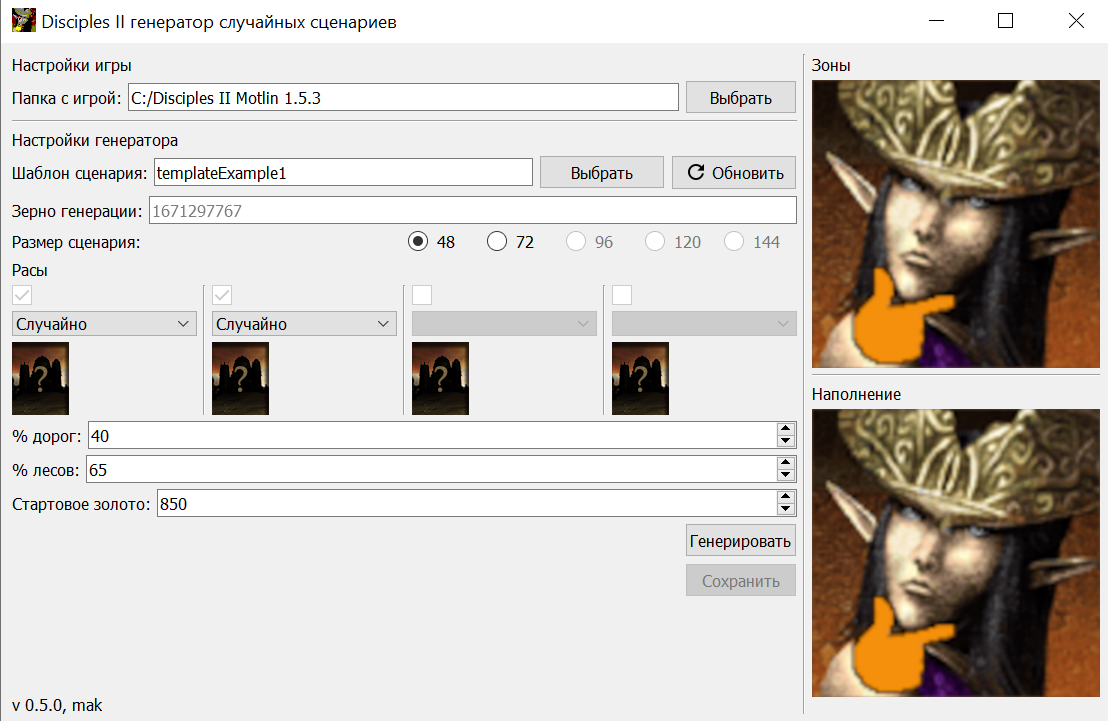
\includegraphics[width=.8\linewidth]{docImages/exampleTemplateLoaded.png}
\caption{Программа генератора с загруженным шаблоном}
\end{figure}

Убедимся что наши дефолтные настроки видны программе и отображены корректно: доступные размеры сценариев, две расы, \% лесов и дорог, стартовое золото.\\
Жмем кнопку \texttt{"Генерировать"} для генерации сценария по шаблону с учетом настроек:

\begin{figure}[H]
\center
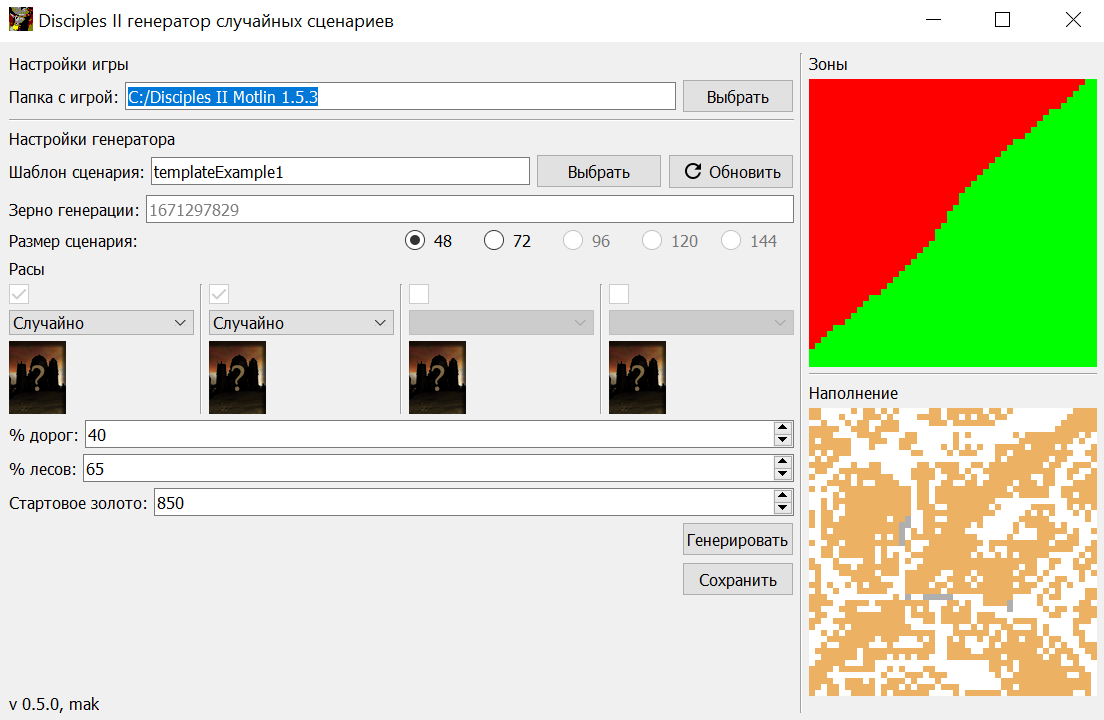
\includegraphics[width=.8\linewidth]{docImages/scenarioGenerated.png}
\caption{Программа с результатами генерации}
\end{figure}

Справа, в окне предпросмотра, видим как карту поделило на две зоны с разными цветовыми индикаторами. В просмотре наполнения видим свободные белые клетки, занятые золотые клетки и клетки дорог, дающие бонус движения, помеченные серым цветом.

Сохраняем сценарий в папку \texttt{Exports} мода, который был выбран и смотрим результаты в редакторе:

\begin{figure}[H]
\center
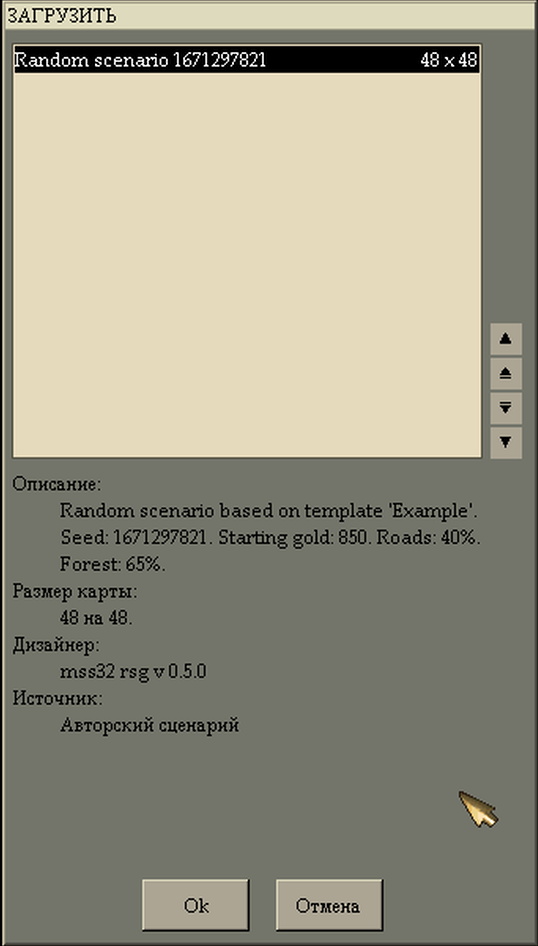
\includegraphics[width=.48\linewidth]{docImages/scenarioInEditor.png}
\caption{Сгенерированный сценарий в редакторе карт}
\end{figure}

Открываем сценарий и смотрим глобальную карту, а также мини-карту:

\begin{figure}[H]
\center
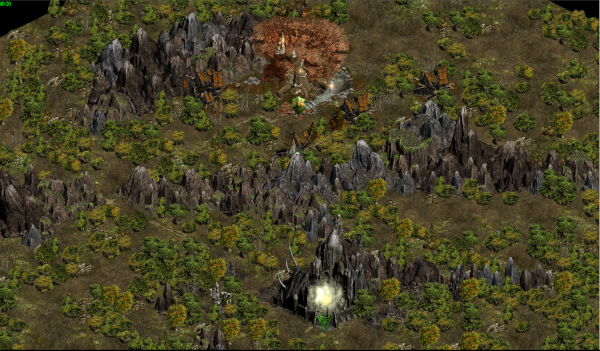
\includegraphics[width=1.0\linewidth]{docImages/scenarioMap.png}
\caption{Случайная карта в редакторе}
\end{figure}

\begin{figure}[H]
\center
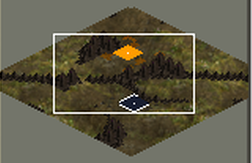
\includegraphics[width=.48\linewidth]{docImages/scenarioMinimap.png}
\caption{Миникарта}
\end{figure}

Убеждаемся что результаты совпадают с описанием в шаблоне: два игрока, каждый в своей зоне. Зоны соединены одним проходом. Поскольку при генерации были выбраны случайные расы, генератор выбрал для сценария Эльфов и Орды нежити.
\newpage
\subsection{Добавляем источники ресурсов}
Начнем наполнение зон в нашем шаблоне с источников ресурсов. Заранее определимся что каждая стартовая зона будет содержать 2 золотые шахты и два источника родной маны. Одна из двух золотых шахт и один источник будут под контролем игрока со старта, остальные придется разведать и захватить в процессе игры.

Поскольку игрок может выбрать любые расы для создания сценария, нам как авторам шаблона нужно учесть это и контроллировать наполнение зон, выбирая тип источников маны с учетом выбранных рас. В этом нам также поможет список рас, поданный в функцию \texttt{getContents}.

Для удобства нашей разработки шаблона и соблюдения правила с рудниками мы вынесем их описание в отдельную функцию, которую будем использовать в описании обеих зон.
Назовем функцию \texttt{getMines} для понимания ее смысла в дальнейшем.
Функция принимает расу игрока в стартовой зоне \texttt{race} и на основании нее вернет таблицу с \hyperref[crystals]{источниками ресурсов} для зоны.
Количество золотых шахт одинаково для обеих стартовых зон, поэтому мы можем сразу указать их в локальной таблице:

\begin{figure}[H]
\lstinputlisting[firstnumber=1, firstline=1, lastline=7]{docExamples/templateExample2.lua}
\caption{Функция для описания источников ресурсов}
\end{figure}

Таблица создается локально внутри функции, а затем после наполнения данными возвращается с помощью директивы \texttt{return}. Такой формат описания выбран только для наглядности. Таблицу источников можно объявить после директивы \texttt{return} и сразу наполнить содержимым, не создавая локально.

Вызываем нашу функцию при описании содержимого каждой из стартовых зон, подавая расу игрока. Таким образом правила генерации источников будут одинаковы для обеих зон даже после изменения логики функции:

\begin{figure}[H]
\lstinputlisting[firstnumber=28, firstline=28, lastline=28]{docExamples/templateExample2.lua}
\lstinputlisting[firstnumber=36, firstline=36, lastline=36]{docExamples/templateExample2.lua}
\caption{Источники ресурсов в стартовых зонах}
\end{figure}

Полный текст шаблона выглядит так:

\begin{figure}[H]
\lstinputlisting{docExamples/templateExample2.lua}
\caption{Заготовка шаблона с золотыми шахтами}
\end{figure}

Сгенерируем карту на основе этого шаблона и убедимся что каждая зона содержит две золотые шахты, расположенные случайно:

\begin{figure}[H]
\center
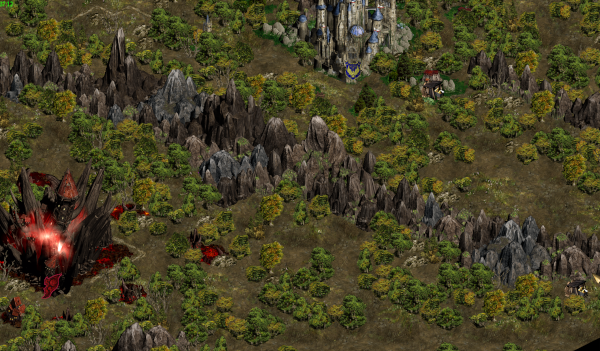
\includegraphics[width=1.0\linewidth]{docImages/scenarioWithMines.png}
\caption{Сценарий с золотыми шахтами}
\end{figure}

На миникарте видны все 4 золотые шахты, по 2 в каждой стартовой зоне:

\begin{figure}[H]
\center
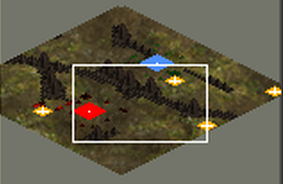
\includegraphics[width=.48\linewidth]{docImages/scenarioMinimapWithMines.png}
\caption{Миникарта с золотыми шахтами}
\end{figure}

На момент когда код функций \texttt{getContents} и \texttt{getMines} будет обработан программой генератора, список рас, присутствующих в сценарии, полностью определен, поэтому нам нужно учитывать только играбельные \hyperref[raceTypes]{расы}. Проверим каждую из 5 рас и добавим в таблицу 2 источника нужного типа:

\begin{figure}[H]
\lstinputlisting[firstnumber=1, firstline=1, lastline=19]{docExamples/templateExample3.lua}
\caption{Выбор источников ресурсов по расе игрока}
\end{figure}

Полный текст шаблона выглядит так:

\begin{figure}[H]
\lstinputlisting{docExamples/templateExample3.lua}
\caption{Шаблон с источниками ресурсов}
\end{figure}

Результаты генерации, в этот раз нам выпали Горные Кланы и Эльфы. Два источника маны рун в зоне кланов и два источника лесного эликсира у эльфов видны на миникарте:

\begin{figure}[H]
\center
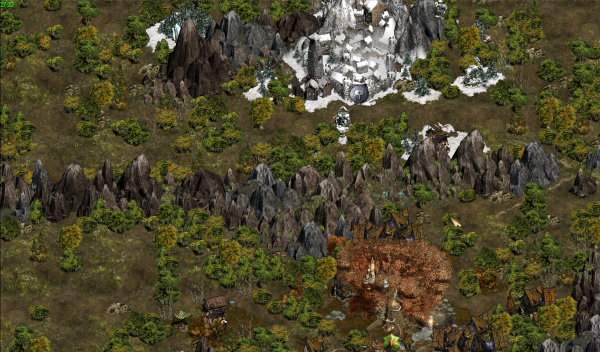
\includegraphics[width=1.0\linewidth]{docImages/scenarioWithMines2.png}
\caption{Сценарий с источниками ресурсов}
\end{figure}

\begin{figure}[H]
\center
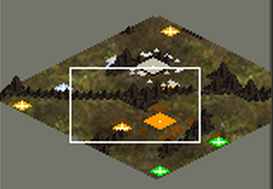
\includegraphics[width=.48\linewidth]{docImages/scenarioMinimapWithMines2.png}
\caption{Миникарта с источниками ресурсов}
\end{figure}
\newpage
\subsection{Добавляем нейтральные города}
Добавим в шаблон нейтральные города. В качестве примера будем создавать разное количество городов в зависимости от размера сценария: один город для размера 48 и два города для 72. Сценарий размера 48 будет содержать город Т2, а сценарий 72 города Т3 и Т5.

Поскольку правило одинаково для двух зон опишем логику городов также отдельной функцией с названием \texttt{getTowns}. Согласно описанию зоны, поле \texttt{towns} представляет собой \textbf{список} описаний городов. В нашем случае список будет содержать одно описание для сценария размером 48 и два описания для 72:

\begin{figure}[H]
\lstinputlisting[firstnumber=1, firstline=1, lastline=12]{docExamples/templateExample4.lua}
\end{figure}

Авторы шаблонов в праве выносить логику в функции и называть их по своему усмотрению.

Не забываем вызывать нашу новую функци в описаниях стартовых зон, передавая размер сценария выбранный пользователем:

\begin{figure}[H]
\lstinputlisting[firstnumber=54, firstline=54, lastline=54]{docExamples/templateExample4.lua}
\lstinputlisting[firstnumber=63, firstline=63, lastline=63]{docExamples/templateExample4.lua}
\end{figure}

Поскольку в описаниях городов отсутствуют гарнизоны, посещающие отряды или лут, мы получаем пустые города как и ожидалось:

\begin{figure}[H]
\center
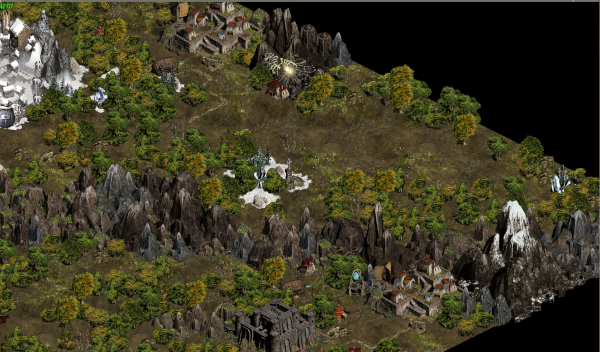
\includegraphics[width=1.0\linewidth]{docImages/scenario48Towns.png}
\caption{Города в сценарии размером 48}
\end{figure}

\begin{figure}[H]
\center
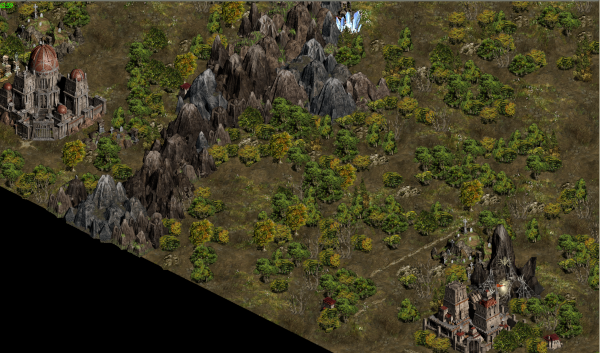
\includegraphics[width=1.0\linewidth]{docImages/scenario72Towns.png}
\caption{Города в сценарии размером 72}
\end{figure}

Теперь когда мы убедились в правильности нашей логики для двух размеров сценариев, можно добавить в города охрану и награды. В гарнизоне Т2 города может быть максимум 2 юнита, посадим туда волков и зеленокожих общей ценностью 200 опыта:

\begin{figure}[H]
\lstinputlisting[firstnumber=4, firstline=4, lastline=11]{docExamples/templateExample5.lua}
\end{figure}

В город Т3 добавим посещающий отряд из варваров и нейтральных людей на 500 опыта, а гарнизон оставим пустым. В качестве награды за захват города положим в инвентарь гарнизона 3 - 4 эликсира восстановления (лечение на 100 хп):

\begin{figure}[H]
\lstinputlisting[firstnumber=13, firstline=13, lastline=26]{docExamples/templateExample5.lua}
\end{figure}

Как упоминалось в самом начале, порядок задания полей в таблицах не играет роли.

В город Т5 добавим отряд из нейтральных людей и эльфов на 500 опыта, а защитников в гарнизоне выберем из жителей болот и нейтралов. Тоже на 500 опыта. В качестве награды посещающий отряд будет владеть одним эликсиром всевышнего (+10\% хп перманентно). В инвентарь гарнизона положим драгоценностей общей суммой 2000 и диапазоном ценности каждой вещи от 250 до 750 золотых. На моде Мотлина версии 1.5.3 такой диапазон ценности должен наполнить инвентарь гарнизона бронзовыми и серебряными кольцами, а также изумрудами. Других типов драгоценностей в награде быть не должно:

\begin{figure}[H]
\lstinputlisting[firstnumber=28, firstline=28, lastline=48]{docExamples/templateExample5.lua}
\end{figure}

Проверим результаты создав сценарий размером 72.\\
Города Т3:

\begin{figure}[H]
\begin{center}
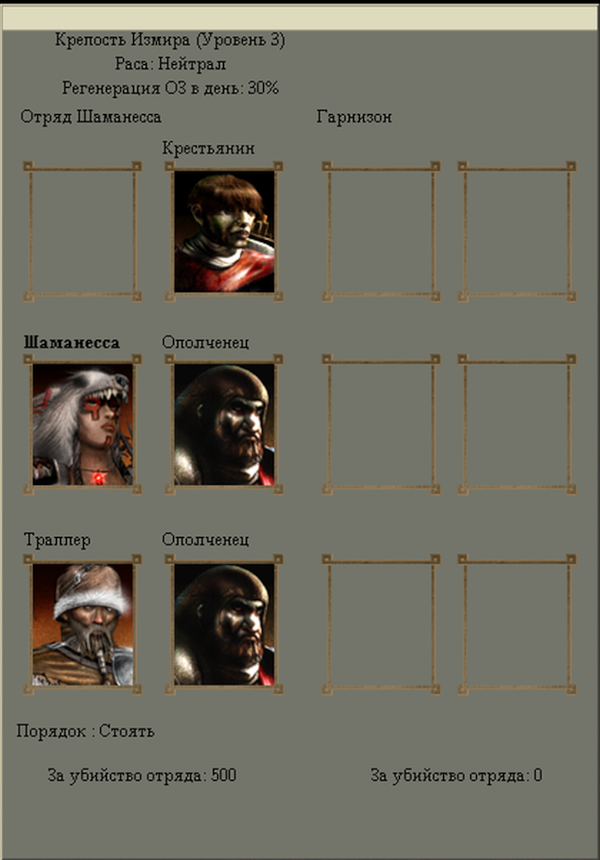
\includegraphics[width=.45\linewidth]{docImages/townT3Preview.png}
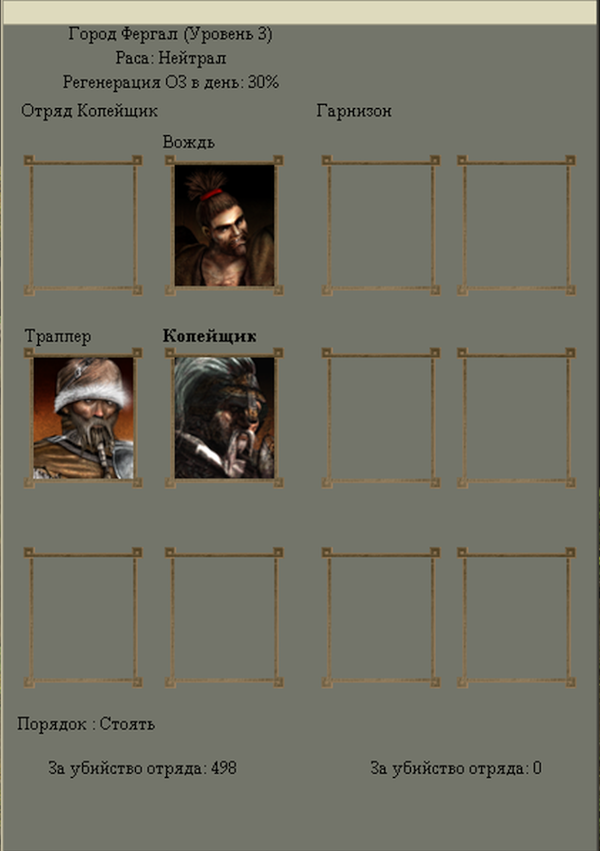
\includegraphics[width=.45\linewidth]{docImages/townT3Preview2.png}
\caption{Просмотр Т3 городов}
\end{center}
\end{figure}

Информация об опыте за убийство отрядов говорит нам о том, что посещающие отряды сгенерировались корректно: близко к 500 опыта в сумме и с учетом заданных субрас.

Проверим инвентари городов:

\begin{figure}[H]
\center
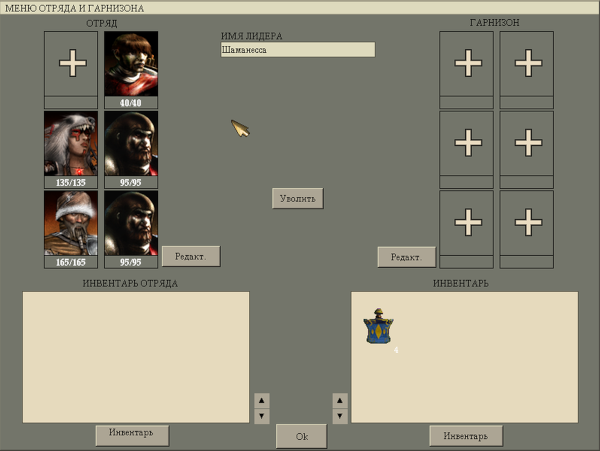
\includegraphics[width=1.0\linewidth]{docImages/townT3Loot.png}
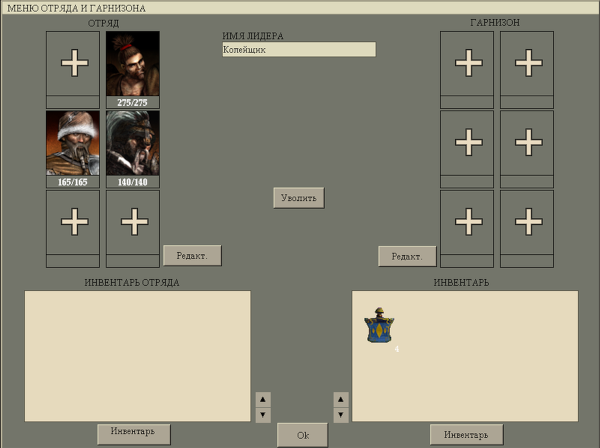
\includegraphics[width=1.0\linewidth]{docImages/townT3Loot2.png}
\caption{Награды Т3 городов}
\end{figure}

Эликсиры восстановления лежат в инвентарях гарнизонов, как и было задумано в шаблоне.

Проверим результаты генерации Т5 городов:

\begin{figure}[H]
\begin{center}
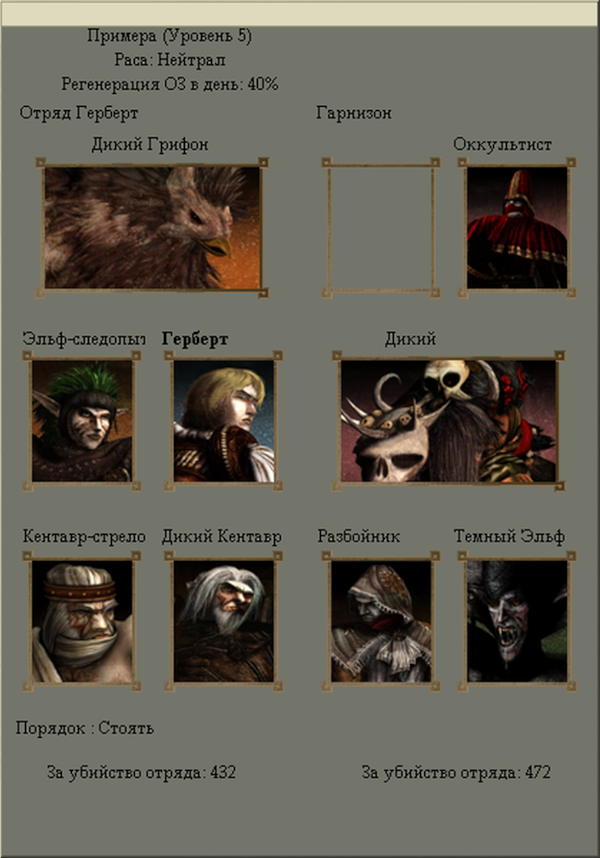
\includegraphics[width=.45\linewidth]{docImages/townT5Preview.png}
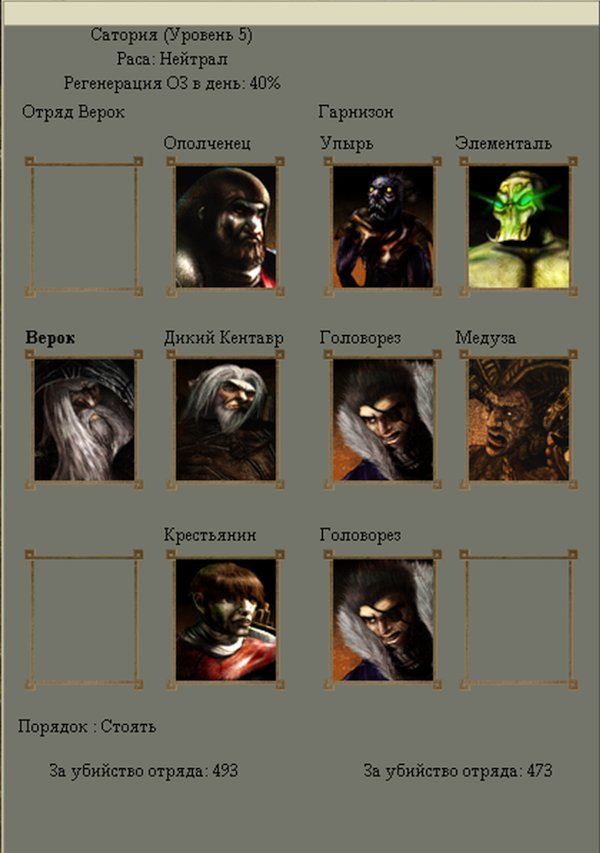
\includegraphics[width=.45\linewidth]{docImages/townT5Preview2.png}
\caption{Просмотр Т5 городов}
\end{center}
\end{figure}

Есть небольшой разброс ценности, но отряды и их субрасы созданы согласно описанию шаблона.

Смотрим инвентари Т5 городов:

\begin{figure}[H]
\center
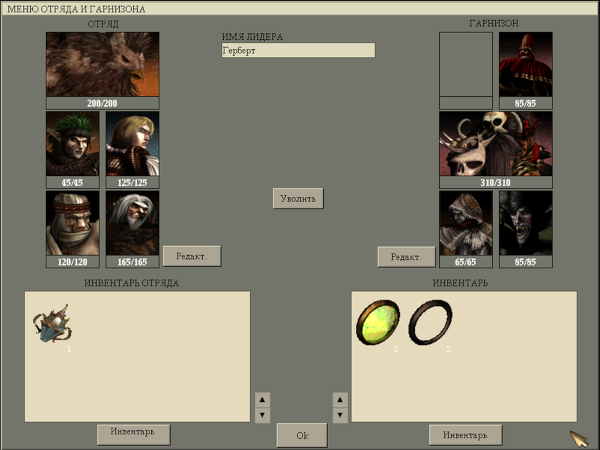
\includegraphics[width=1.0\linewidth]{docImages/townT5Loot.png}
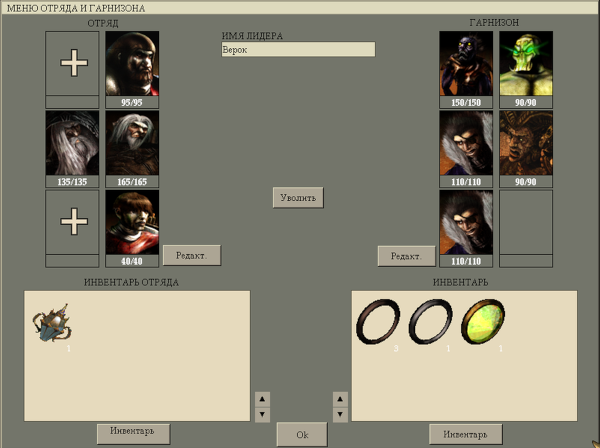
\includegraphics[width=1.0\linewidth]{docImages/townT5Loot2.png}
\caption{Награды Т5 городов}
\end{figure}

Как видим перманентные зелья на месте, а драгоценности в гарнизонах собраны лишь из двух видов колец и изумрудов в случайных пропорциях, но согласно общей сумме. Все согласно описанию шаблона.

Полный текст функции \texttt{getTowns}:

\begin{figure}[H]
\lstinputlisting[firstnumber=1, firstline=1, lastline=52]{docExamples/templateExample5.lua}
\end{figure}

Полный текст шаблона, а также другие примеры шаблонов идут вместе с программой генератора и этой документацией.
\newpage

\end{document}